% !TeX root = RJwrapper.tex
\title{\pkg{OpenLand}: Software for Quantitative Analysis and Visualization of Land
Use and Cover Change}
\author{by Reginal Exavier and Peter Zeilhofer}

\maketitle

\abstract{%
There is an increasing availability of spatially explicit, freely
available land use and cover (LUC) time series worldwide. Because of the
enormous amount of data this represents, the continuous updates and
improvements in spatial and temporal resolution and category
differentiation, as well as increasingly dynamic and complex changes
made, manual data extraction and analysis is highly time consuming, and
making software tools available to automatize LUC data assessment is
becoming imperative. This paper presents a software developed in R,
which combines LUC raster time series data and their transitions,
calculates state-of-the-art LUC change indicators, and creates
spatio-temporal visualizations, all in a coherent workflow. The
functionality of the application developed is demonstrated using an LUC
dataset of the Pantanal floodplain contribution area in Central Brazil.
}

\hypertarget{introduction}{%
\subsection{Introduction}\label{introduction}}

Land use and land cover (LUC) monitoring provides key information on the
ecological state and biophysical properties of the land surface and is
widely used in climatic, hydrological, and ecological modelling
\citep{Brovkin2013, Verburg2015}. Global population growth over the last
decades has led to increased rates of LUC change (LUCC), which has
affected all major ecosystem services, including biodiversity, climate,
and water supply, and has altered carbon cycling
\citep{Ballantyne2015, Nelson2010, Song2018}.

The importance of these applications is supported by the continuous
expansion of remote sensing data acquisition programs, making freely
available an increasing amount of spatially explicit LUC time series
data worldwide \citep{Prestele2016}. The huge volume of these datasets,
their timely actualization, ever-increasing spatial resolution and
category differentiation, and a variety of data formats, render their
manual extraction and analysis increasingly time consuming. This is
especially true when trying to compare or harmonize LUC datasets of the
same study area generated from different sources, with different
methodological approaches across different spatial and temporal scales,
in order to output the factual LUC in a region of interest
\citep{Yang2017}.

Human interference on LUC is complex, and the intensity and frequency of
LUC transitions are increasing. Therefore, the development of sound LUC
models is highly dependent on a deep understanding of past and ongoing
LUCC processes \citep{Muller2014}. This means that LUC patterns have to
be constantly reviewed to underpin our understanding of these processes
\citep{Lambin1997, Lambin2006}, develop a baseline analysis for
projections of future LUC \citep{Hurtt2011}, and to construct, calibrate
and validate LUCC simulations \citep{Prestele2016}. Such efforts require
tools for data extraction, pre-processing, visualization, and
calculation of LUC metrics to relieve the burden from labour-intensive
and time-consuming manual data processing and analysis \citep{Yu2019a}.
If the procedures implemented to do so follow standards in land cover
characterization, and use formalized methodological approaches in LUC
analysis, the resulting analytics become more transparent, robust, and
auditable \citep{Herold2006, Muller2014, Yang2017}.

\citet{Aldwaik2012} developed an approach called Intensity Analysis
(IA), which examines changes in LUC categories by comparing the
intensity of change between categories during a given time interval with
a hypothesized uniform change intensity. Since then, several case
studies have emphasized the potential of Intensity Analysis to
synthetize complex LUCC under different spatial and temporal scales,
such as urban environments \citep{Akinyemi2017, Subasinghe2016},
regional studies \citep{Melo2018, Mwangi2017, Souza2017}, and
country-wide comparisons \citep{Chaudhuri2016}. Furthermore,
\citet{Huang2018} concluded that intensity analysis metrics outperform
other indicators of land use dynamics in the comparison between
candidate regions, while \citet{Varga2019} showed that IA metrics are a
helpful tool for assessing the quality of LUC modelling outputs.

In IA, the uniform change intensity of a time period is compared with
the observed intensities of transitions between LUC categories. The
calculations are carried out using transition matrices between LUC
categories, assessing specific: (i) time intervals, (ii) categories or
classes and (iii) types of transitions. The first assessment level
examines in which time intervals global annual change rates are faster,
slower or comparable to an average rate of change. The second level
determines which category transitions are relatively dormant or more
active within a given time interval, based on an analysis of gross
change. The gross gains and losses for each category in a given time
interval are compared with an averaged, uniform annual change. The third
level of assessment seeks to identify which transitions are particularly
intensive during the time interval considered. In order to do so each
transition is compared with a uniform transition intensity. The
mathematical notations used for the IA indicators measuring size and
intensities of temporal changes among LUC categories (Equations 1-8) can
be found in \citet{Aldwaik2012} and \citet{Aldwaik2013}.

Analytical tools for the analysis of LUC time series are commonly
available in compiled languages and distributed as software packages or
extensions to proprietary geographic information systems such as ArcGIS
or Idrisi \citep{Moulds2015}. Consequently, the source code for such
tools, used for land use change analysis and modelling, is often
unavailable \citep{Rosa2014}. This makes adopting the applications of
new approaches and reproducing scientific results difficult
\citep{Morin2012, Peng2011}. GIS software has made widely available
spatially explicit visualization capabilities for multi-temporal LUC,
which is crucial for documentation and analysis of LUC distribution.
However, maps can become blurred and non-interpretable when extensive
time series or complex landscapes with different category transitions
need to be analysed. This is particularly true when multi-category
changes have to be analysed at multiple time steps to improve the
understanding of landscape processes, in which case non-spatial forms of
LUCC will have to be explored.

By contrast, the availability of packages to perform analyses of LUC
categories in time series data is limited. \CRANpkg{intensity.analysis}, developed
by \citet{PontiusJr.2019}, is an application of IA, with functionality
limited to the calculation of the three IA assessment levels described
above and their plotting; this package does not allow any
personalization. Little pre-processing capability is available. If
needed, input rasters cannot be checked for spatial and thematic
consistency, and they have to be manually imported to R and stored. No
other commonly used LUC metrics can be calculated or plotted. Tools to
visualize LUC changes are limited to standard plots of the three IA
analysis levels. lulccR \citep{Moulds2015} is another package developed
for LUC change analysis and focuses on the application of tools for LUC
change modelling.

This highlights the need for flexible and comprehensive tools for
multipurpose analyses of complex LUC time series data. This paper aims
to demonstrate that we have developed a solution, available as freeware,
which allows the agile consistency analysis, extraction, pre-processing,
analysis, and visualization of multiresolution time series data in a
straightforward workflow, thereby increasing productivity in information
extraction for an improved understanding of LUCC processes at different
spatial scales. Originating primarily from the application of the
intensity analysis method, the formatted tabular representation of
multiple transition steps can be a valuable tool to support the quick
calculation of LUCC indicators.

\hypertarget{conceptual-overview}{%
\subsection{Conceptual Overview}\label{conceptual-overview}}

The software was developed to provide comprehensive support for LUCC
analysis over time and implement the intensity analysis conceptual
approach proposed by \citet{Aldwaik2012}, and further described in
\citet{Aldwaik2013}.

The source language of the \CRANpkg{OpenLand} package \citep{Exavier2020} is R,
and it was conceived using the integrated development environment (IDE)
RStudio \citep{RStudioTeam2016}. For full functionality, \pkg{OpenLand}
depends on selected, third-party functions of the \CRANpkg{raster},
\CRANpkg{dplyr} and \CRANpkg{tidyr} R packages
\citep{Hijmans2019, Wickham2019, Wickham2019a} (Fig.
\ref{fig:conception}). Visualization tools make use of \CRANpkg{ggplot2},
\CRANpkg{circlize}, \CRANpkg{ComplexHeatmap}, \CRANpkg{gridExtra} and
\CRANpkg{networkD3} R packages
\citep{Allaire2017, Auguie2017, Gu2014, Wickham2016}. Designed
as an iterative workflow, the pre-processing of a raw LUC time series is
followed by the extraction and visualization of single or multistep LUC
transitions and/or a complete IA.

\begin{Schunk}
\begin{figure}[h]

{\centering 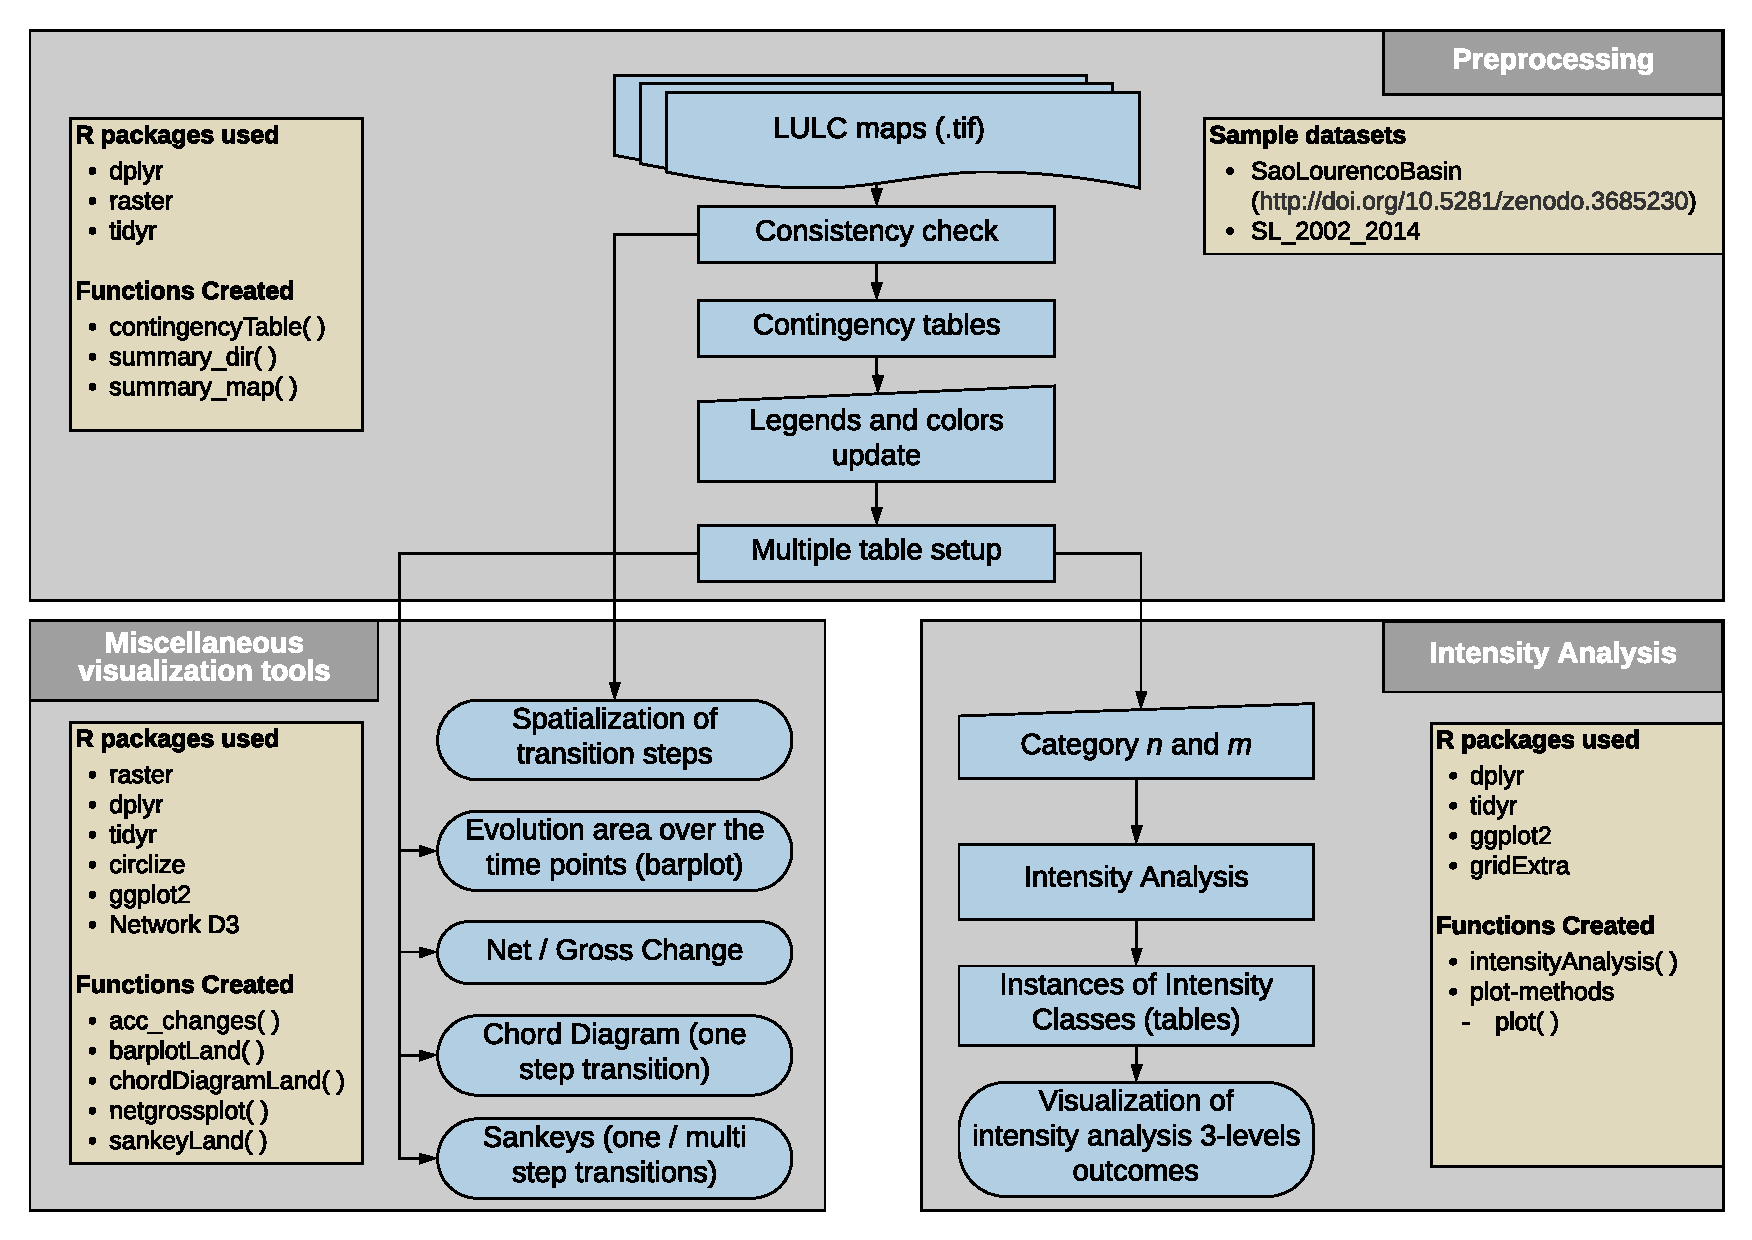
\includegraphics[width=0.8\linewidth,]{figures/conception_overview.pdf} 

}

\caption[Conceptual overview of the OpenLand package showing reused R functionalities]{Conceptual overview of the OpenLand package showing reused R functionalities.}\label{fig:conception}
\end{figure}
\end{Schunk}

The main processing workflow should begin with a consistency check of
the input files, which have to be a sequence of LUC maps in a tif format
(Fig. \ref{fig:conception}). In the following step, a contingency table
of LUC transitions for each time step can be calculated. Two
complementary analysis workflows are then available. First, a set of
miscellaneous non-spatial visualization tools allows for a quick
screening of LUC dynamics. Second, a complete intensity analysis
\citep{Aldwaik2012, Aldwaik2013} can be implemented, including tools to
visualize change intensities over time, category and transition levels.
Ancillary functionalities include allow for extraction and spatial
visualization of LUCC frequencies.

\hypertarget{functionality-and-implementation}{%
\subsection{Functionality and
Implementation}\label{functionality-and-implementation}}

\hypertarget{the-suxe3o-lourenuxe7o-river-basin-example-dataset}{%
\subsubsection{The São Lourenço River Basin Example
Dataset}\label{the-suxe3o-lourenuxe7o-river-basin-example-dataset}}

The \pkg{OpenLand} functionality is demonstrated using an LUC dataset of the
São Lourenço river basin, of major importance to the Pantanal wetland
into which it flows. The data is as provided in the
4\textsuperscript{th} edition of the
\href{https://www.embrapa.br/pantanal/bacia-do-alto-paraguai}{Monitoring
of Changes in Land cover and Land Use in the Upper Paraguay River Basin
- Brazilian portion - Review Period: 2012 to 2014}
\citep{Embrapapantanalsite2015}, and the time series is composed of five
LUC maps (2002, 2008, 2010, 2012 and 2014). The study area is located in
the Cerrado savanna biome, in the southeastern corner of the Brazilian
state of Mato Grosso, and covers approximately 22,400
km\textsuperscript{2}. Some level of LUCC has occurred in about 12\% of
the area over the past 12 years, including some deforestation and
intensification of existing agricultural uses. In order to be processed
using the \pkg{OpenLand} package, the original multi-year shapefile was
clipped to the extent of the São Lourenço basin, transformed into
rasters and saved as a 5-layer \texttt{RasterStack}; it is available
from a public repository
\href{https://zenodo.org/record/3685230\#.Xl7cDMgReUk}{(https://doi.org/10.5281/zenodo.3685229)}
as an \texttt{.RDA} file which can be loaded into R.

\begin{Schunk}
\begin{Sinput}
# Installing the released version of OpenLand from CRAN
install.packages("OpenLand")

# Loading the OpenLand package
library(OpenLand)

# downloading the SaoLourencoBasin multi-layer raster and make it available into R
url <- "https://zenodo.org/record/3685230/files/SaoLourencoBasin.rda?download=1"

temp <- tempfile()
download.file(url, temp, mode = "wb")
load(temp)

# looking on the metadata of the example dataset
SaoLourencoBasin 
\end{Sinput}
\begin{Soutput}
#> class      : RasterStack 
#> dimensions : 6372, 6546, 41711112, 5  (nrow, ncol, ncell, nlayers)
#> resolution : 30, 30  (x, y)
#> extent     : 654007.5, 850387.5, 8099064, 8290224  (xmin, xmax, ymin, ymax)
#> crs        : +proj=utm +zone=21 +south +ellps=GRS80 +units=m +no_defs 
#> names      : landscape_2002, landscape_2008, landscape_2010, landscape_2012, landscape_2014 
#> min values :              2,              2,              2,              2,              2 
#> max values :             13,             13,             13,             13,             13
\end{Soutput}
\end{Schunk}

To visualize the output of the LUC analysis in \pkg{OpenLand}, we simplified
the legend of the original dataset and used the following 11 LUC
categories for the basin: forest formation (FF), three Cerrado savanna
formations (SF, SA, SG), anthropogenized vegetation (aa), i.e.~mostly
altered Cerrado formations used for grazing, composed of natural
species, cattle farming (Ap), crop farming (Ac), mining areas (Im),
urban areas (Iu), water bodies (Agua), and reforestation (R) (Table
\ref{tab:legend_table}).

\begin{table}[htbp]
\centering
\caption{The original legend from SOS Pantanal.}
\label{tab:legend_table}
\begin{tabular}[t]{llllll}
\hline
Pixel Value & Legend & Class      & Category                    & Colour \\
\hline
2        & Ap     & Anthropogenic & Cattle farming              & \#FFE4B5 \\
3        & FF     & Natural       & Forest  formation           & \#228B22 \\
4        & SA     & Natural       & Park savanna                & \#00FF00 \\
5        & SG     & Natural       & Gramineous savanna          & \#CAFF70 \\
7        & aa     & Anthropogenic & Anthropogenized vegetation  & \#EE6363 \\
8        & SF     & Natural       & Wooded savanna              & \#00CD00 \\
9        & Agua   & Natural       & Water bodies                & \#436EEE \\
10       & Iu     & Anthropogenic & Urban areas                 & \#FFAEB9 \\
11       & Ac     & Anthropogenic & Crop farming                & \#FFA54F \\
12       & R      & Anthropogenic & Reforestation               & \#68228B \\
13       & Im     & Anthropogenic & Mining areas                & \#636363 \\
\hline
\end{tabular}
\end{table}

\hypertarget{consistency-check-and-data-extraction-from-raster-time-series}{%
\subsubsection{Consistency Check and Data Extraction from Raster Time
Series}\label{consistency-check-and-data-extraction-from-raster-time-series}}

Two auxiliary functions allow users to check for consistency in the
input gridded LUC time series, including extent, projection, cell
resolution and categories. The \texttt{summary\_map()} function returns
the number of pixels in each category for each single raster layer,
whereas the summary\_dir() function lists the spatial extent, spatial
resolution, cartographic projection and the category range of a set of
LUC maps.

For the initial spatial screening of the time series, the acc\_changes()
function determines the number of LUC transitions during the entire time
interval of the series. The results of percentage area by transition
frequencies in the study area are stored in a table and a grid layer is
generated, which can be plotted (Fig. \ref{fig:acchange}) using for
example the \texttt{tmap} package.

\begin{Schunk}
\begin{Sinput}
# the acc_changes() function, with the SaoLourencoBasin dataset
SL_changes <- acc_changes(SaoLourencoBasin)
SL_changes
\end{Sinput}
\begin{Soutput}
#> [[1]]
#> class      : RasterLayer 
#> dimensions : 6372, 6546, 41711112  (nrow, ncol, ncell)
#> resolution : 30, 30  (x, y)
#> extent     : 654007.5, 850387.5, 8099064, 8290224  (xmin, xmax, ymin, ymax)
#> crs        : +proj=utm +zone=21 +south +ellps=GRS80 +units=m +no_defs 
#> names      : layer 
#> values     : 0, 2  (min, max)
#> 
#> 
#> [[2]]
#> # A tibble: 3 x 3
#>   PxValue       Qt Percent
#>     <int>    <int>   <dbl>
#> 1       0 21819779   87.6 
#> 2       1  2787995   11.2 
#> 3       2   301086    1.21
\end{Soutput}
\end{Schunk}

\begin{Schunk}
\begin{figure}[h]

{\centering 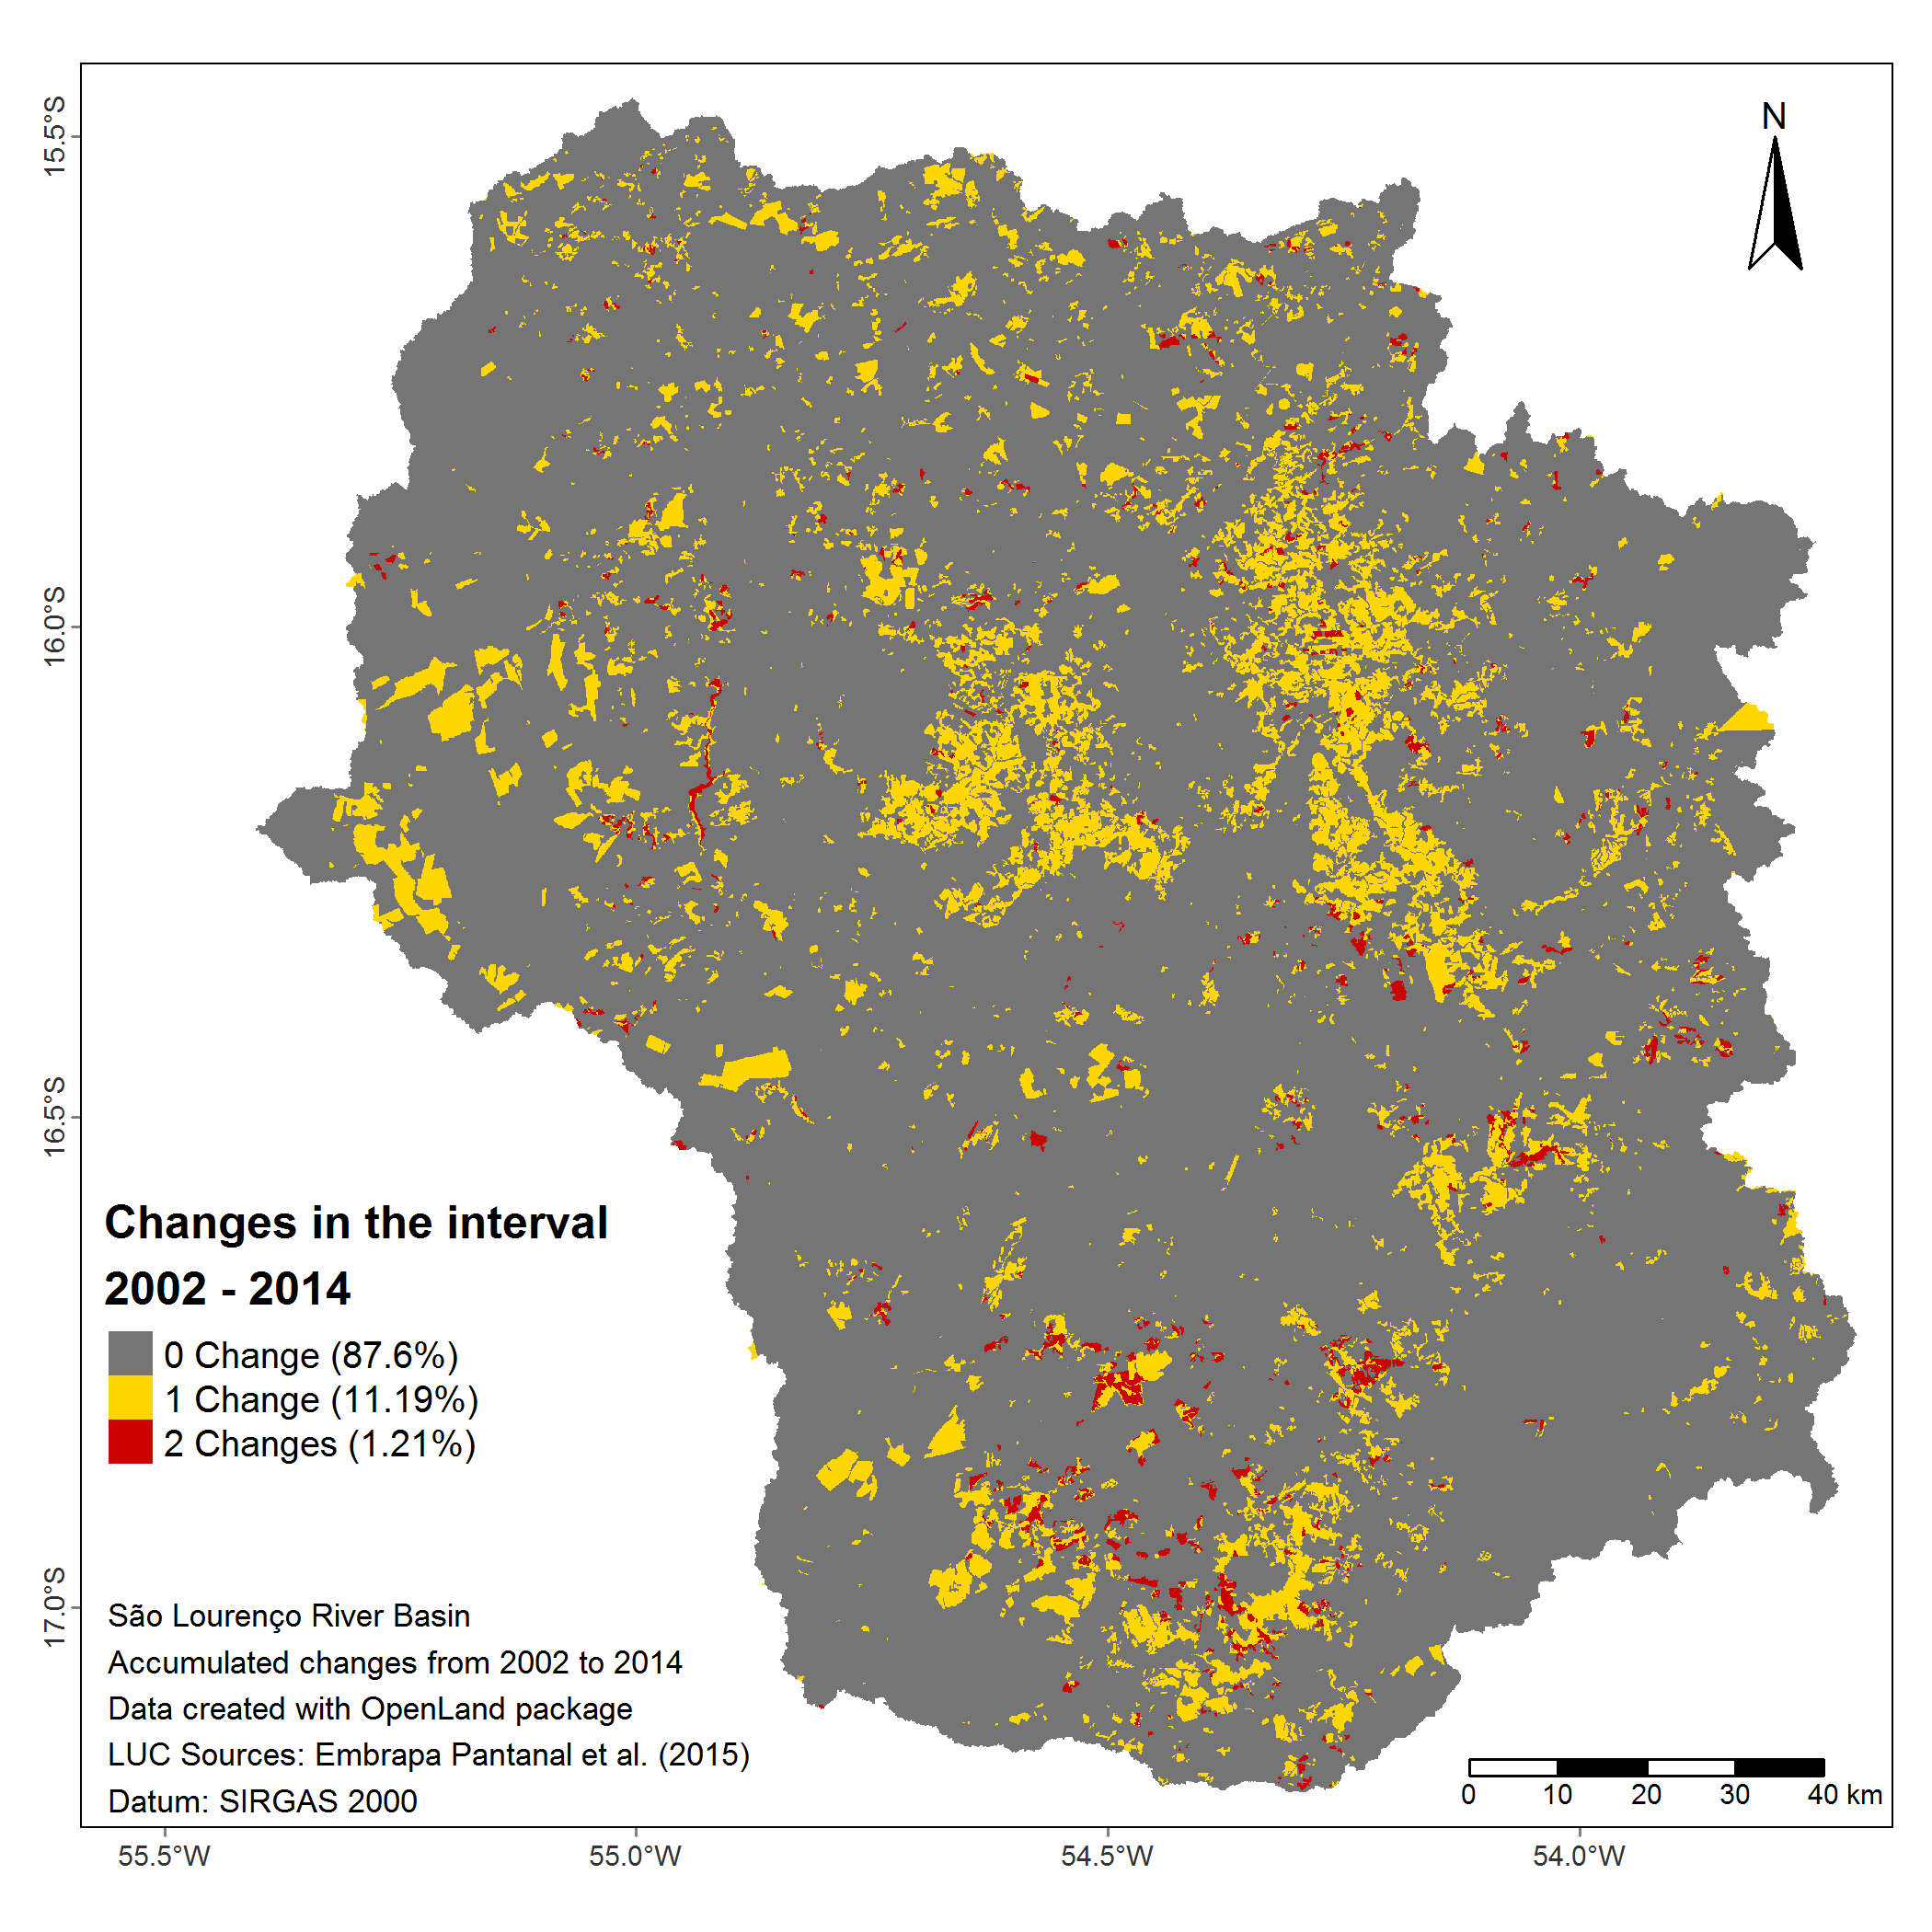
\includegraphics[width=0.7\linewidth,]{figures/acc_mymap.png} 

}

\caption[Accumulated changes in pixels in the interval 2002 - 2014 at four time points (2002, 2008, 2010, 2012, 2014)]{Accumulated changes in pixels in the interval 2002 - 2014 at four time points (2002, 2008, 2010, 2012, 2014).}\label{fig:acchange}
\end{figure}
\end{Schunk}

As most deforestation occurred in the 20th century, unchanged areas
totalled 87.6\%. Approximately 35\% of the watershed had already been
deforested in 1985, versus 46\% in 2014 \citep{Mapbiomas}. 11.19\%
showed a unique alteration and 1.21\% a two-folded alteration for the
five time points of the input series considered. All further analytical
and visualization tools are based on the contingencyTable() function,
which builds a matrix of transitions between LUC categories according to
the temporal resolution of the original time series. Multiple grid
scanning by contingencyTable() returns 5 objects: lulc\_Multistep,
lulc\_Onestep, tb\_legend, totalArea, totalInterval. The first two
objects are contingency tables; the first (lulc\_Multistep) takes into
account the grid cells of the entire time series, whereas the second
(lulc\_Onestep) calculates LUC transitions only between the first and
last year of the series. The third object (tb\_legend) is a table
containing the category name associated with pixel values and a colour
scheme. As category values and colours are initially created randomly,
their values must be edited to produce meaningful plot legends and
colour schemes. The fourth object (totalArea) is a table containing the
extent of the study area in km\textsuperscript{2} and in pixel units.
The fifth table (totalInterval) stores the range of years between the
first (Y\textsubscript{t=1}) and last year (Y\textsubscript{T}) of the
series. Table \ref{tab:prototype} presents the fields created, together
with their format, description and labelling as per a table output by
the contingencyTable function.

\begin{table}[htbp]
\centering
\caption{Prototype contingency table.}
\label{tab:prototype}
\begin{tabular}[t]{>{\centering}p{0.10\columnwidth}<{\small}>{\centering}p{0.08\columnwidth}<{\small}>{\centering}p{0.08\columnwidth}<{\small}>{\small}p{0.12\columnwidth}<{\centering}>{\small}p{0.12\columnwidth}<{\centering}>{\small}p{0.10\columnwidth}<{\centering}>{\small}p{0.08\columnwidth}<{\centering}>{\small}p{0.08\columnwidth}<{\centering}}
\toprule
\([Y_t,Y_{t+1}]\) & Category\(_i\) & Category\(_j\) & C\(_{tij}\) (km\(^2\)) & C\(_{tij}\) (pixel) & \(Y_{t+1} - Y_t\) & \(Y_t\) & \(Y_{t+1}\) \\
\midrule
chr & int & int & dbl & int & int & int & int \\

Period of analysis from time point \textit{t} to time point \textit{t+1} & A category at interval's initial time point & A category at  interval's final time point & Number of elements in km\(^2\) that transits from category \textit{i} to category \textit{j} & Number of elements in pixel that transits from category \textit{i} to category \textit{j} & Interval in years between time point \textit{t} and time point \textit{t+1} & Initial Year of the interval & Final Year of the interval \\
\textbf{Period} & \textbf{From} & \textbf{To} & \textbf{km2} & \textbf{QtPixel} & \textbf{Interval} & \textbf{yearFrom} & \textbf{yearTo} \\
\bottomrule
\end{tabular}
\end{table}

As mentioned, the \textbf{tb\_legend} object must be edited with the
real category names and colours associated with the category values. In
our case, the category names and colours follow the conventions given by
\citep{sospantanal2015}
\href{https://www.embrapa.br/documents/1354999/1529097/BAP+-+Mapeamento+da+Bacia+do+Alto+Paraguai+-+estudo+completo/e66e3afb-2334-4511-96a0-af5642a56283}{(access
document here, page 17)} like the values in (Table
\ref{tab:legend_table}).

\begin{Schunk}
\begin{Sinput}
## creating the contingency table
SL_2002_2014 <- contingencyTable(input_raster = SaoLourencoBasin,
                                 pixelresolution = 30)
names(SL_2002_2014)
\end{Sinput}
\begin{Soutput}
#> [1] "lulc_Multistep" "lulc_Onestep"   "tb_legend"      "totalArea"     
#> [5] "totalInterval"
\end{Soutput}
\begin{Sinput}
## editing the category names
SL_2002_2014$tb_legend$categoryName <- factor(c("Ap", "FF", "SA", "SG", "aa", "SF", 
                                                "Agua", "Iu", "Ac", "R", "Im"),
                                     levels = c("FF", "SF", "SA", "SG", "aa", "Ap", 
                                                "Ac", "Im", "Iu", "Agua", "R"))

## adding the colours by the same order of the legend
SL_2002_2014$tb_legend$color <- c("#FFE4B5", "#228B22", "#00FF00", "#CAFF70", 
                                  "#EE6363", "#00CD00", "#436EEE", "#FFAEB9", 
                                  "#FFA54F", "#68228B", "#636363")
\end{Sinput}
\end{Schunk}

\FloatBarrier

\hypertarget{miscellaneous-non-spatial-visualization-tools}{%
\subsection{Miscellaneous Non-Spatial Visualization
Tools}\label{miscellaneous-non-spatial-visualization-tools}}

\hypertarget{evolution-of-luc-areas}{%
\paragraph{Evolution of LUC areas}\label{evolution-of-luc-areas}}

Exploratory data analysis based on the \texttt{contingencyTable()}
function may begin with the visualization of the absolute and/or
percentage area of each LUC category at each time point using a grouped
bar plot (Fig. \ref{fig:evolution_plot}), in order to show the evolution
of the LUC categories at each time point of the series.

\begin{Schunk}
\begin{Sinput}
barplotLand(dataset = SL_2002_2014$lulc_Multistep, 
            legendtable = SL_2002_2014$tb_legend,
            xlab = "Year",
            ylab = bquote("Area (" ~ km^2~ ")"),
            area_km2 = TRUE)
\end{Sinput}
\begin{figure}[htbp]

{\centering 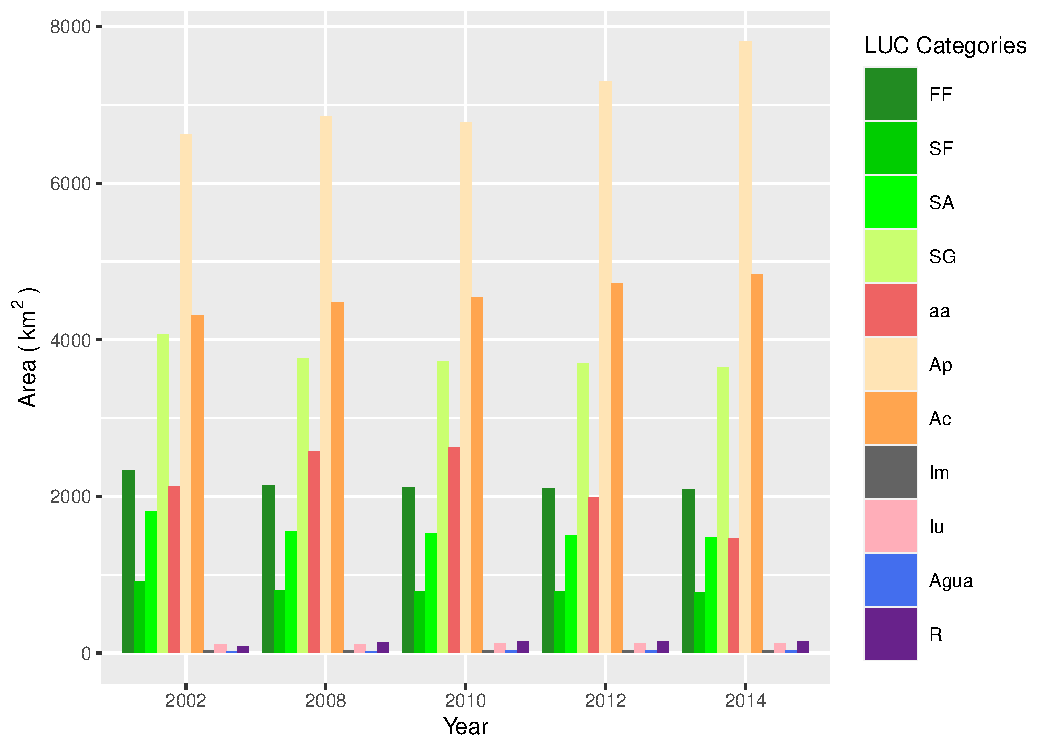
\includegraphics[width=0.7\linewidth,]{figures/barplotLand.pdf} 

}

\caption[LUC evolution Bar Plot 2002 – 2014]{LUC evolution Bar Plot 2002 – 2014.}\label{fig:evolution_plot}
\end{figure}
\end{Schunk}

\hypertarget{net-and-gross-changes}{%
\paragraph{Net and gross changes}\label{net-and-gross-changes}}

For the analysis of long time series with high temporal resolution,
information extraction from evolution bar plots may become demanding and
alterations between categories through time points are only as net
changes. For a category-wise, simultaneous assessment of net and gross
changes, multistep transitions can be balanced through a stacked bar
chart (Fig. \ref{fig:ng_plot}). In the São Lourenço river basin, all
natural vegetation categories suffered an equal net and gross loss (FF,
SF, SA, SG) between 2002 and 2014. In contrast, mining (Im) and
urbanized (Iu) areas as well as waterbodies (Agua) and reforestation (R)
had equal amounts of net and gross gains. Principally anthropogenized
vegetation (aa) and pastures showed differences in net and gross
changes, pointing to more complex underlying LUCC processes.

\begin{Schunk}
\begin{Sinput}
netgrossplot(dataset = SL_2002_2014$lulc_Multistep,
             legendtable = SL_2002_2014$tb_legend,
             xlab = "LUC Category",
             ylab = bquote("Area (" ~ km^2 ~ ")"),
             changesLabel = c(GC = "Gross changes", NG = "Net Gain", NL = "Net Loss"),
             color = c(GC = "gray70", NG = "#006400", NL = "#EE2C2C"), 
             area_km2 = TRUE)
\end{Sinput}
\begin{figure}[h]

{\centering 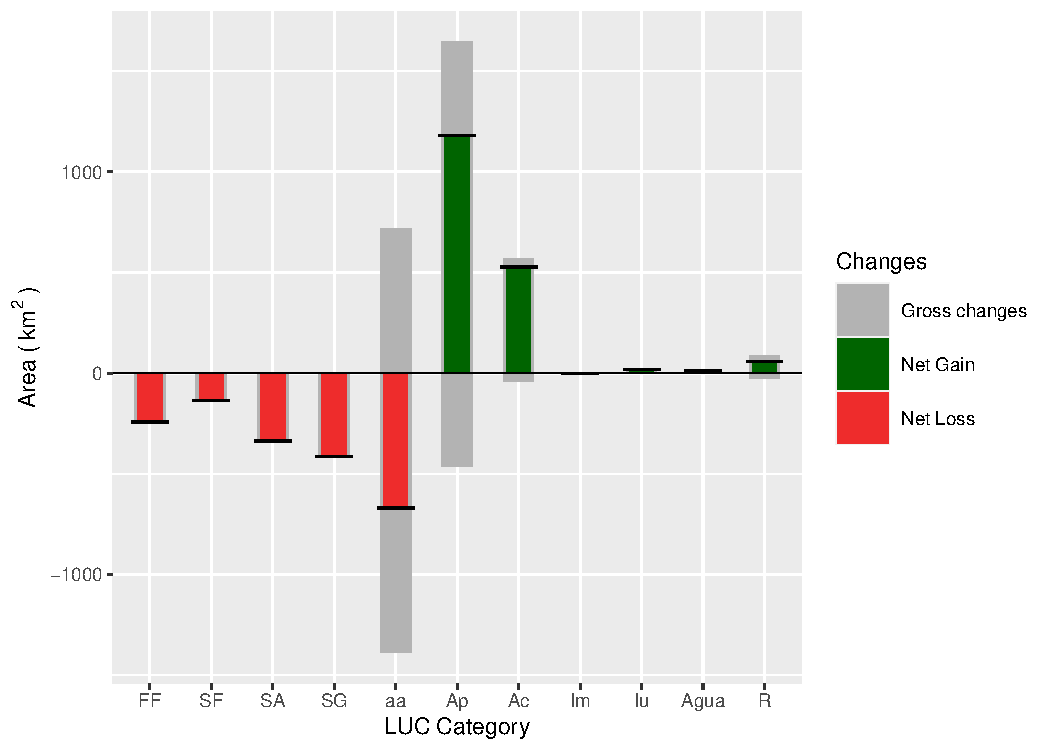
\includegraphics[width=0.8\linewidth, height=0.5\linewidth]{figures/net_gross.pdf} 

}

\caption[Net Gross Changes 2002 - 2014]{Net Gross Changes 2002 - 2014.}\label{fig:ng_plot}
\end{figure}
\end{Schunk}

To further explore specifically those non-linear transitions,
single-step Chord (Fig. \ref{fig:chordDiagram}) and Sankey diagrams
(Fig. \ref{fig:sankeys1} and \ref{fig:sankeys2}) can be composed for
each time point in the series. Considering the entire observation
period, the major gross change was from anthropogenized areas (aa) to
cattle farming (Ap). Both the Chord and Sankey diagrams show however
that pastures did not directly gain from clear-cut deforestation, but
from the previous degradation of natural vegetation categories
principally until 2008 (FF, SF, SA, SG), and a subsequent transition
from aa to Ap between 2010 and 2014.

\hypertarget{chord-diagram-2002-2014}{%
\paragraph{Chord Diagram (2002 -- 2014)}\label{chord-diagram-2002-2014}}

\begin{Schunk}
\begin{Sinput}
chordDiagramLand(dataset = SL_2002_2014$lulc_Onestep,
                 legendtable = SL_2002_2014$tb_legend,
                 area_km2 = TRUE)
\end{Sinput}
\begin{figure}[h]

{\centering 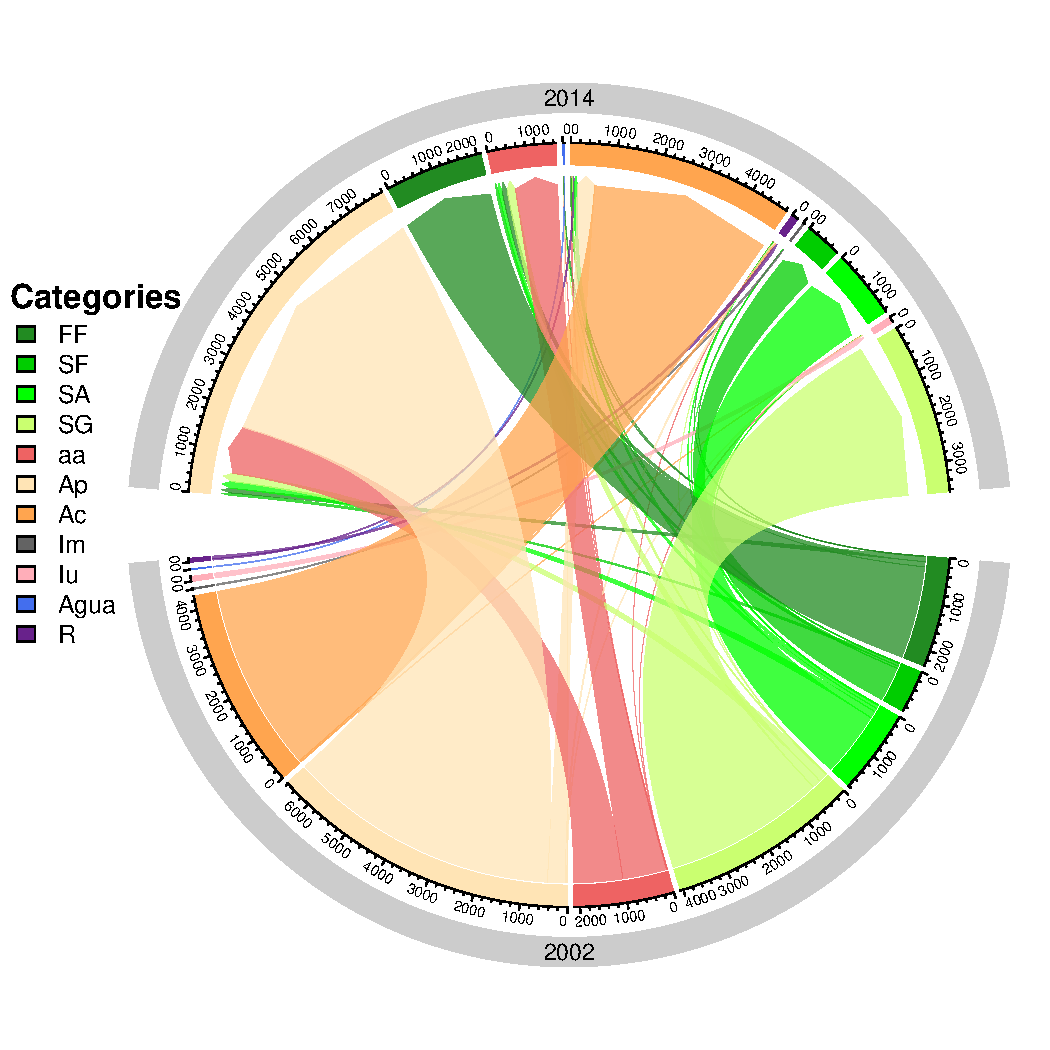
\includegraphics[width=0.8\linewidth,]{figures/chordDiagram.pdf} 

}

\caption[Chord Diagram 2002 - 2014]{Chord Diagram 2002 - 2014.}\label{fig:chordDiagram}
\end{figure}
\end{Schunk}

\hypertarget{single-step-sankey-diagram-2002-2014}{%
\paragraph{Single-step Sankey diagram (2002 --
2014)}\label{single-step-sankey-diagram-2002-2014}}

\begin{Schunk}
\begin{Sinput}
# sankeyLand(dataset = SL_2002_2014$lulc_Onestep,
#            legendtable = SL_2002_2014$tb_legend)
\end{Sinput}
\end{Schunk}

\begin{Schunk}
\begin{figure}[htbp]

{\centering \subfloat[Onestep transition 2002 - 2014\label{fig:sankeys1}]{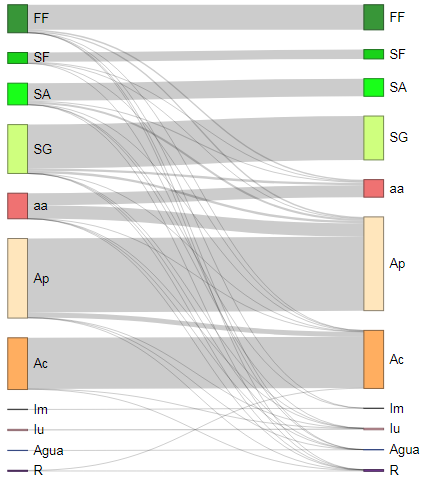
\includegraphics[width=0.5\linewidth,height=0.3\textheight,]{figures/sankey_one.png} }\subfloat[Multistep transition 2002-2008-2010-2012-2014\label{fig:sankeys2}]{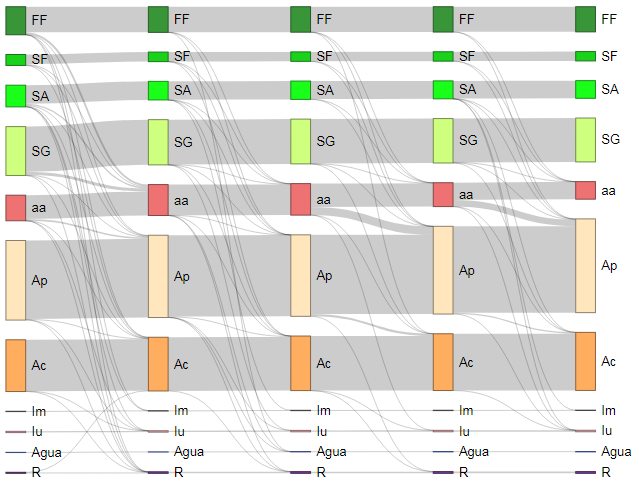
\includegraphics[width=0.5\linewidth,height=0.3\textheight,]{figures/sankey_multi.png} }

}

\caption[Sankeys Plot 2002 - 2014]{Sankeys Plot 2002 - 2014}\label{fig:sankeys}
\end{figure}
\end{Schunk}

\hypertarget{multistep-sankey-diagram}{%
\paragraph{Multistep Sankey diagram}\label{multistep-sankey-diagram}}

If between-category transitions have to be visualized simultaneously for
the entire time series, a multistep version of the Sankey plot can be
output (Fig. \ref{fig:sankeys2}).

\begin{Schunk}
\begin{Sinput}
# sankeyLand(dataset = SL_2002_2014$lulc_Multistep,
#            legendtable = SL_2002_2014$tb_legend)
\end{Sinput}
\end{Schunk}

\hypertarget{intensity-analysis}{%
\subsection{Intensity Analysis}\label{intensity-analysis}}

Intensity Analysis (IA) is a quantitative method for the analysis of LUC
maps over several time steps, using cross-tabulation matrices, where
each matrix summarizes the LUC change for each time interval. IA
evaluates the deviation between observed change intensity and
hypothesized uniform change intensity in three levels. Thereby, each
level details information given by the previous analysis level. First,
the \textbf{interval level} indicates how the size and rate of change
vary over time intervals. Second, the \textbf{category level} examines
for each time interval how the size and intensity of gross losses and
gross gains in each category vary across categories for each time
interval. Third, the \textbf{transition level} determines the size and
intensity of each transition from one category to another during each
time interval. At each level, the method also tests for stationarity of
patterns across time intervals \citep{Aldwaik2012}. In the \pkg{OpenLand}
package, the \texttt{intensityAnalysis()} function computes the three
levels of analysis. It requires the object returned by the
\texttt{contingenceTable()} function and that the user predefines two
LUC categories \texttt{n} and \texttt{m}. Generally, \texttt{n} is a
target category that experienced relevant gains and \texttt{m} a
category with important losses.

\begin{Schunk}
\begin{Sinput}
testSL <- intensityAnalysis(dataset = SL_2002_2014, category_n = "Ap",
                            category_m = "SG", area_km2 = TRUE)

# it returns a list with 6 objects
names(testSL)
\end{Sinput}
\begin{Soutput}
#> [1] "lulc_table"           "interval_lvl"         "category_lvlGain"    
#> [4] "category_lvlLoss"     "transition_lvlGain_n" "transition_lvlLoss_m"
\end{Soutput}
\end{Schunk}

The \texttt{intensityAnalysis()} function returns 6 objects:
lulc\_table, interval\_lvl, category\_lvlGain, category\_lvlLoss,
transition\_lvlGain\_n, transition\_lvlLoss\_m. The object-oriented
approach adopted here allowed us to set specific methods for plotting
the intensity objects. Specifically, we used the S4 class, which
requires the formal definition of classes and methods
\citep{Chambers2008}. The first object is a contingency table similar to
the lulc\_Multistep object with the unique difference that the columns
\texttt{From} and \texttt{To} are replaced by their appropriate
denominations in the LUC legend.

The second object \emph{\textbf{interval\_lvl}} is an \texttt{Interval}
object, the third \emph{\textbf{category\_lvlGain}} and the fourth
\emph{\textbf{category\_lvlLoss}} are \texttt{Category} objects, while
the fifth \emph{\textbf{transition\_lvlGain\_n}} and the
\emph{\textbf{transition\_lvlLoss\_m}} are \texttt{Transition} objects.

An \texttt{Interval} object has one slot containing a table of the
\textbf{interval level} results (\emph{(S\textsubscript{t} equation
(\ref{eq:st}) and U equation (\ref{eq:U}) values)}. A \texttt{Category}
object has three slots: the first contains the colour associated with
the legend item as name attribute, the second slot contains a table of
the \textbf{category level} results \emph{(gain (G\textsubscript{tj})
equation (\ref{eq:gtj}) or loss (L\textsubscript{ti}) equation
(\ref{eq:lti}) values)}, and the third slot contains a table storing the
results of a stationarity test. A \texttt{Transition} object also has
three slots: the first contains the colour associated with the
respective legend item defined as name attribute, the second slot
contains a table of the \textbf{transition level} results \emph{(gain n
(R\textsubscript{tin} equation (\ref{eq:rtin}) and W\textsubscript{tn}
equation (\ref{eq:wtn})) or loss m (Q\textsubscript{tmj} equation
(\ref{eq:qtmj}) and V\textsubscript{tm} equation (\ref{eq:vtm}))
values)}. The third slot contains a table storing the results of a
stationarity test. \citet{Aldwaik2012} consider a case stationary only
when the intensities for all time intervals are on one side of the
uniform intensity, i.e.~they are consistently either smaller or larger
than the uniform rate over the entire period.

\begin{equation} \label{eq:st}
S_t = \frac{\sum_{j=1}^{J} \left[( \sum_{i=1}^{J} C_{tij}) - C_{tij} \right]}{(Y_{t+1} - Y_{t})\left(\sum_{j=1}^{J} \sum_{i=1}^{J} C_{tij}\right)} \times 100\%
\end{equation}

\begin{equation} \label{eq:U}
U = \frac{\sum_{t=1}^{T-1} \left\{(Y_{t+1} - Y_t) \sum_{j=1}^{J} \left[\left(\sum_{i=1}^{J} C_{tij}\right) - C_{tjj}   \right]\right\}}{(Y_{T} - Y1) \sum_{t=1}^{T-1} \left[(Y_{t+1} - Y_t) \left(\sum_{j=1}^{J} \sum_{i=1}^{J} C_{tij}\right)  \right]} \times 100\%
\end{equation}

\begin{equation} \label{eq:gtj}
G_{tj} = \frac{\left[\left( \sum_{i=1}^{J} C_{tij} \right) - C_{tjj}   \right] / (Y_{t+1} - Y_t)}{\sum_{i=1}^{J} C_{tij})} \times 100\%
\end{equation}

\begin{equation} \label{eq:lti}
L_{ti} = \frac{\left[\left( \sum_{j=1}^{J} C_{tij} \right) - C_{tii}   \right] / (Y_{t+1} - Y_t)}{\sum_{j=1}^{J} C_{tij})} \times 100\%
\end{equation}

\begin{equation} \label{eq:rtin}
R_{tin} = \frac{C_{tin} / (Y_{t+1} - Y_t)}{\sum_{j=1}^{J} C_{tij})} \times 100\%
\end{equation}

\begin{equation} \label{eq:wtn}
W_{tn} = \frac{\left[\left( \sum_{i=1}^{J} C_{tin} \right) - C_{tnn}   \right] / (Y_{t+1} - Y_t)}{\sum_{j=1}^{J}  \left[\left( \sum_{i=1}^{J} C_{tij} \right) - C_{tnj}   \right]} \times 100\%
\end{equation}

\begin{equation} \label{eq:qtmj}
Q_{tmj} = \frac{C_{tmj} / (Y_{t+1} - Y_t)}{\sum_{i=1}^{J} C_{tij}} \times 100\%
\end{equation}

\begin{equation} \label{eq:vtm}
V_{tm} = \frac{\left[\left( \sum_{j=1}^{J} C_{tmj} \right) - C_{tmm}   \right] / (Y_{t+1} - Y_t)}{\sum_{i=1}^{J}  \left[\left( \sum_{j=1}^{J} C_{tij} \right) - C_{tim}   \right]} \times 100\%
\end{equation}

\hypertarget{graphs-output-of-the-intensity-analysis}{%
\subsubsection{Graphs (Output of the intensity
analysis)}\label{graphs-output-of-the-intensity-analysis}}

Visualizations of the IA results are obtained with the
\texttt{plot(intensity-object)} method. For more details on the function
arguments, please see the documentation of the \texttt{plot()} method
implemented.

\hypertarget{interval-level}{%
\paragraph{Interval Level}\label{interval-level}}

The IA interval level is a measure of the overall rate of LUC changes
over consecutive time intervals in the series. The plot (Fig.
\ref{fig:int_level}) has two sides: on the left the percentage of change
during the corresponding time step, and on the right the percentage of
change per year showing the reference line of the Uniform rate.

\begin{Schunk}
\begin{Sinput}
plot(testSL$interval_lvl,
     labels = c(leftlabel = "Interval change area (%)",
                rightlabel = "Annual change area (%)"),
     marginplot = c(-8, 0), leg_curv = c(x = .3, y = .1))
\end{Sinput}
\begin{figure}[h]

{\centering 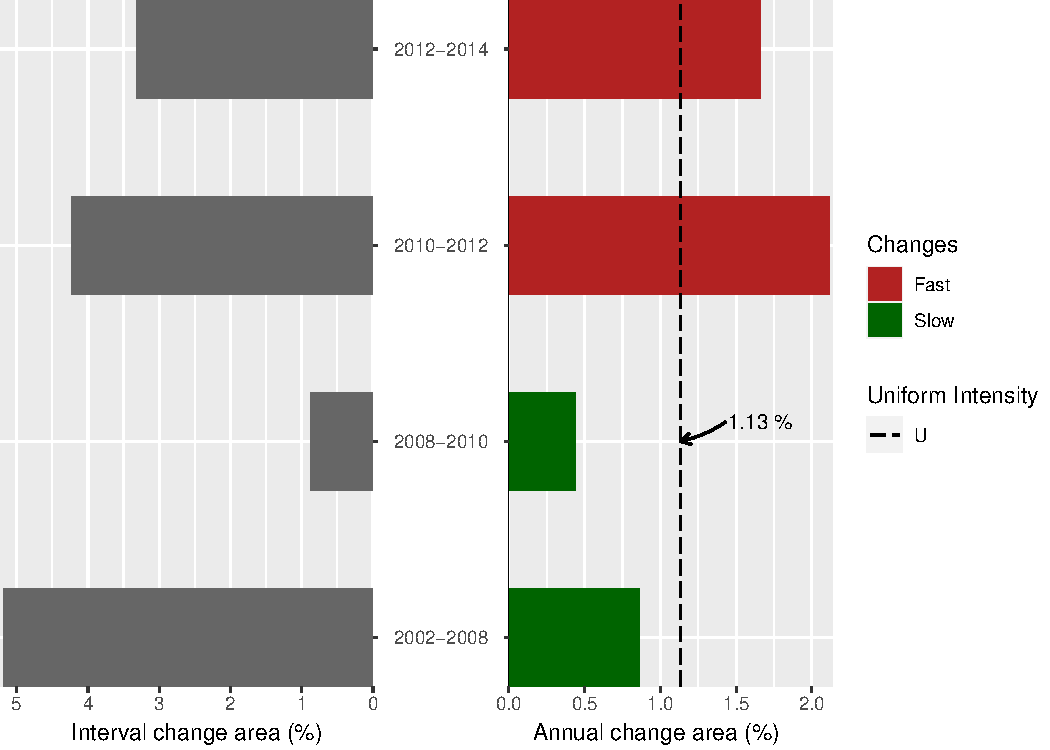
\includegraphics[width=0.6\linewidth,]{figures/interval_lvl.pdf} 

}

\caption[IA Interval Level plot]{IA Interval Level plot.}\label{fig:int_level}
\end{figure}
\end{Schunk}

In the São Lourenço basin, the interval level plot shows that LUC change
has accelerated over the last decade, with a peak between 2010 and 2012,
when the actual rate of change was almost double the Uniform rate. This
recent acceleration in LUC in the Cerrado biome has been interpreted
partially as a spillover effect of conservation efforts in the Amazon
basin \citep{Dou2018}.

\hypertarget{category-level-gain-and-loss-area}{%
\paragraph{Category Level (Gain and Loss
Area)}\label{category-level-gain-and-loss-area}}

After the analysis of LUC change intensity independently from LUC
categories, the category level allows further examination into which
land categories are relatively dormant versus active in a given time
interval and whether this pattern is stable across time intervals
\citep{Aldwaik2012}.

\begin{Schunk}
\begin{Sinput}
# Gain area
plot(testSL$category_lvlGain,
     labels = c(leftlabel = bquote("Gain Area (" ~ km ^ 2 ~ ")"),
                rightlabel = "Intensity Gain (%)"),
     marginplot = c(.3, .3), leg_curv = c(x = 1, y = .5))

# Loss area
plot(testSL$category_lvlLoss,
     labels = c(leftlabel = bquote("Loss Area (" ~ km ^ 2 ~ ")"),
                rightlabel = "Loss Intensity (%)"),
     marginplot = c(.3, .3), leg_curv = c(x = 1, y = .5))
\end{Sinput}
\begin{figure}[htbp]

{\centering \subfloat[Gain area\label{fig:cat_level1}]{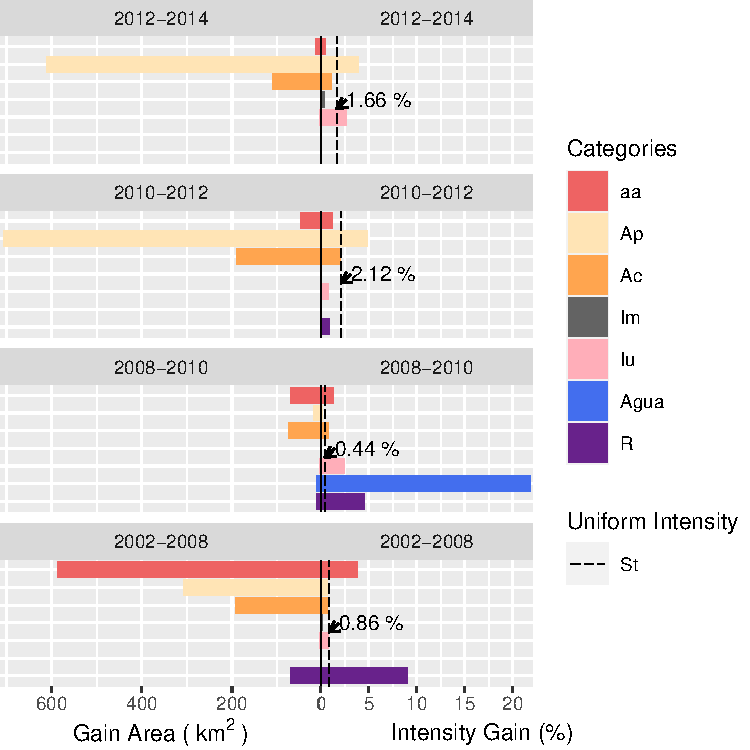
\includegraphics[width=0.5\linewidth,]{figures/category_lvlGain.pdf} }\subfloat[Loss area\label{fig:cat_level2}]{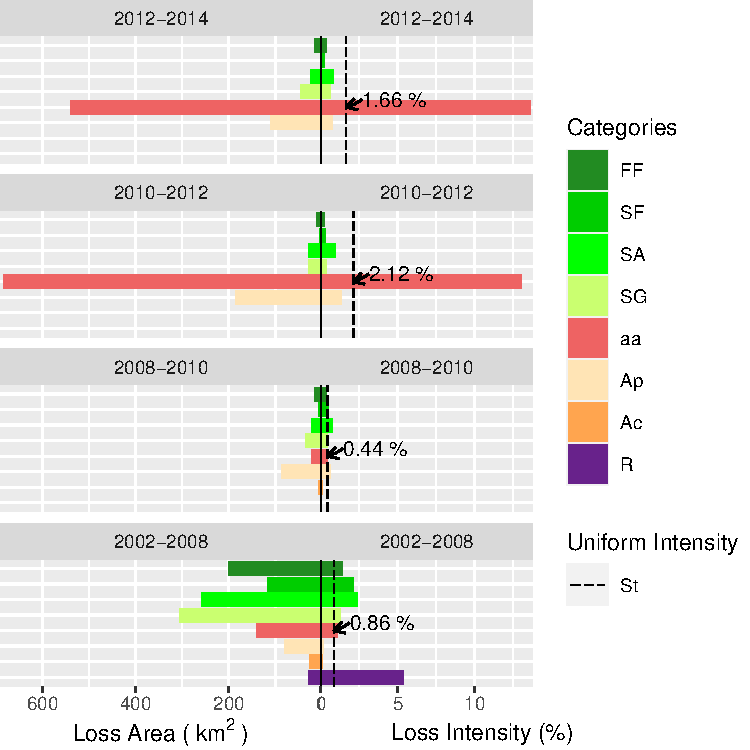
\includegraphics[width=0.5\linewidth,]{figures/category_lvlLoss.pdf} }

}

\caption[IA Category level (a) gain and (b) loss plots]{IA Category level (a) gain and (b) loss plots.}\label{fig:cat_level}
\end{figure}
\end{Schunk}

To facilitate legibility, we chose to split the category level plots
(Fig. \ref{fig:cat_level}) into area gains (Fig. \ref{fig:cat_level1})
and losses (Fig. \ref{fig:cat_level2}). Area gains in land categories R
and aa were more intense over the first six-year period (2002-2008) than
they were at any other subsequent time point. The very intense area gain
in water bodies during the second time interval (2008-2010) corresponds
to the São Lourenço hydropower plant reservoir being filled. In the
third and fourth intervals, the expansion of pasture areas Ap was more
intense than during previous time steps. In parallel, the land category
aa is in sharp decline.

\hypertarget{transition-level-gain-of-the-category-n-ap-and-loss-of-the-category-m-sg}{%
\paragraph{\texorpdfstring{Transition Level (Gain of the category
\texttt{n} ``Ap'' and Loss of the category \texttt{m}
``SG'')}{Transition Level (Gain of the category n ``Ap'' and Loss of the category m ``SG'')}}\label{transition-level-gain-of-the-category-n-ap-and-loss-of-the-category-m-sg}}

In the transition level, the analysis focuses on the intensity of gain
of a particular category \texttt{n} from all the individual categories
in the landscape and/or on the intensity of loss of a particular
category \texttt{m} to all the individual categories in the landscape
for each time interval.

\begin{Schunk}
\begin{Sinput}
# Gain of the category `n` "Ap"
plot(testSL$transition_lvlGain_n,
     labels = c(leftlabel = bquote("Gain of Ap (" ~ km^2 ~ ")"),
                rightlabel = "Intensity Gain of Ap (%)"),
     marginplot = c(.3, .3), 
     leg_curv = c(x = 1, y = .2))

# Loss of the category `m` "SG"
plot(testSL$transition_lvlLoss_m,
     labels = c(leftlabel = bquote("Loss of SG (" ~ km^2 ~ ")"), 
                rightlabel = "Intensity Loss of SG (%)"),
     marginplot = c(.3, .3), 
     leg_curv = c(x = .1, y = .4))
\end{Sinput}
\begin{figure}[htbp]

{\centering \subfloat[Gain of category n (Ap)\label{fig:trans_level1}]{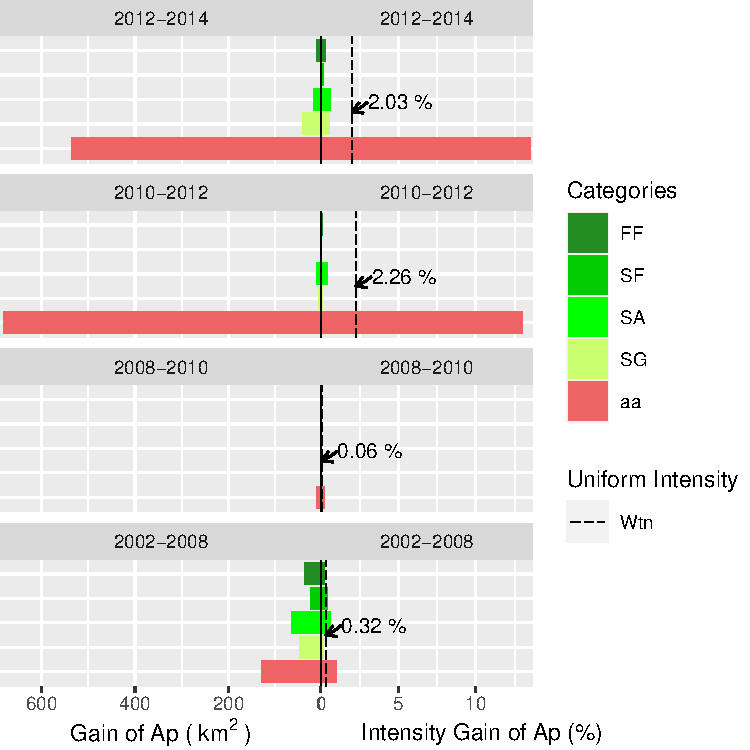
\includegraphics[width=0.5\linewidth,]{figures/transition_lvlGain_n.pdf} }\subfloat[Loss of category m (SG)\label{fig:trans_level2}]{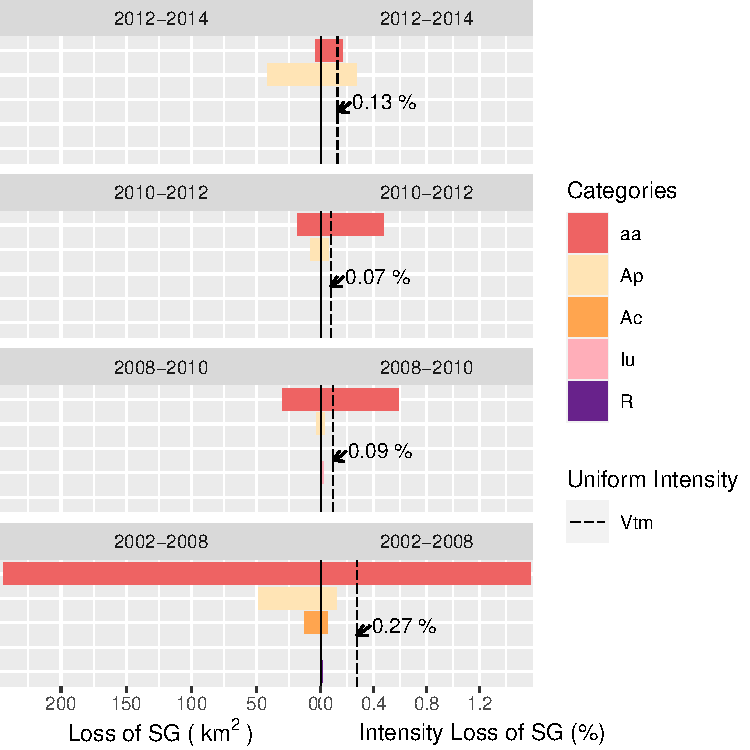
\includegraphics[width=0.5\linewidth,]{figures/transition_lvlLoss_m.pdf} }

}

\caption[IA Transition level plots of Ap gains and SG losses]{IA Transition level plots of Ap gains and SG losses.}\label{fig:trans_level}
\end{figure}
\end{Schunk}

The area gains in the Ap category and losses in the SG category of the
SaoLourencoBasin dataset are used here as an example. Results in (Fig.
\ref{fig:trans_level1}) show that areas in Ap were principally gained
from the aa category, and that this transition was particularly intense
in the third and fourth time periods. Meanwhile, area losses in the SG
savannah formation persisted over the entire span of the time series
(Fig. \ref{fig:trans_level2}). However, there was a change in the land
uses these areas were lost to: during the first three intervals, SG was
lost principally to aa, while in the last time interval, the loss was
more intensely due directly to the Ap category.

\hypertarget{conclusions-and-further-research}{%
\subsection{Conclusions and further
research}\label{conclusions-and-further-research}}

In response to added and refined temporal, spatial and thematic
dimensions increasing the volume of LUC data, the \pkg{OpenLand} package
provides a comprehensive and integrated suite for the exploratory
analysis of LUC changes. It offers seamless processing workflows
beginning with time series consistency checking, data extraction,
analysis and plotting of commonly used LUC metrics, as well as an
implementation of Intensity Analysis, a state-of-the-art top-down
hierarchical methodological framework to quantify the intensity of LUC
changes. Regardless of the complexity of an LUC time series, all
transitions and metrics are automatically extracted, quantified and
stored as objects, without any need for further tabular data
manipulation for analysis. Visualization tools create pre-formatted
print-ready plots, which can be easily modified through function
arguments.

\citet{Aldwaik2013} presented an extension of IA, which allows us to
consider hypothetical classification errors in input LUC maps as part of
the comparison between observed and uniform intensities in IA. The
implementation of their method in\pkg{OpenLand} could further help users to
assess the implications of errors on the strength of the evidence in the
outputs of their Intensity Analysis and therefore, improve their
understanding of LUC change processes.

\hypertarget{acknowledgements}{%
\subsubsection{Acknowledgements}\label{acknowledgements}}

Reginal Exavier is supported by the Brazilian Funding Agency CAPES
(Coordination for the Improvement of Higher Level Personnel) through a
Master studentship (2018 - 2020) at the Department of Geography of the
Federal University of Mato Grosso.

\bibliography{exavier-zeilhofer}


\address{%
Reginal Exavier\\
Department of Geography\\
Federal University of Mato Grosso\\ Avenida Fernando Corrêa da Costa, 2367 -- Boa Esperança, Cuiabá -- MT,
78060-900\\
}
\href{mailto:reginalexavier@rocketmail.com}{\nolinkurl{reginalexavier@rocketmail.com}}

\address{%
Peter Zeilhofer\\
Department of Geography\\
Federal University of Mato Grosso\\ Avenida Fernando Corrêa da Costa, 2367 -- Boa Esperança, Cuiabá -- MT,
78060-900\\
}
\href{mailto:zeilhoferpeter@gmail.com}{\nolinkurl{zeilhoferpeter@gmail.com}}

